     \chapter{Stuff you want to include}

A 1\degree C step input (\SI{35}{\milli\volt}), as shown in figure \ref{fig:ts}, was used to determine the settling time. The settling time is measured at the point where the output steps to 90\% of the final value (\SI{622}{\milli\volt}), which is \SI{560}{\milli\volt}. The settling time was thus measured as \SI{62.07}{ms}, as shown by the cursor difference in figure \ref{ts}.
\begin{figure}[h]
    \centering
    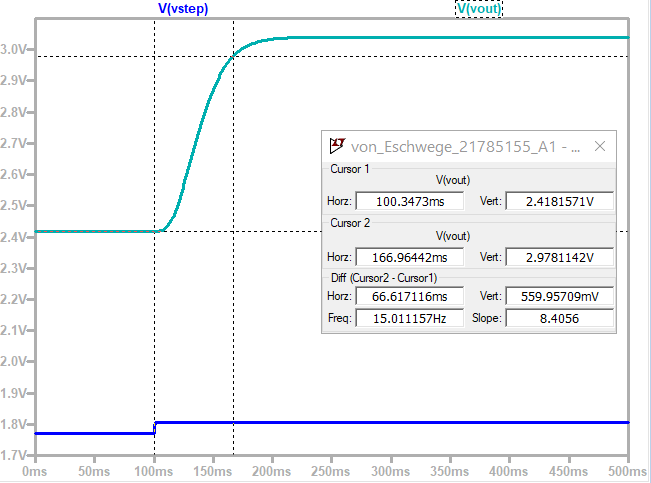
\includegraphics[width = 0.8\textwidth]{Figures/ts.png}
    \caption{Settling Time Measurement}
    \label{fig:ts}
\end{figure}

The bode plot for the low-pass filter is shown in figure \ref{fig:ac}. The -3dB point is lower than calculated, but is still well within the acceptable range. 
\begin{figure}[h]
    \centering
    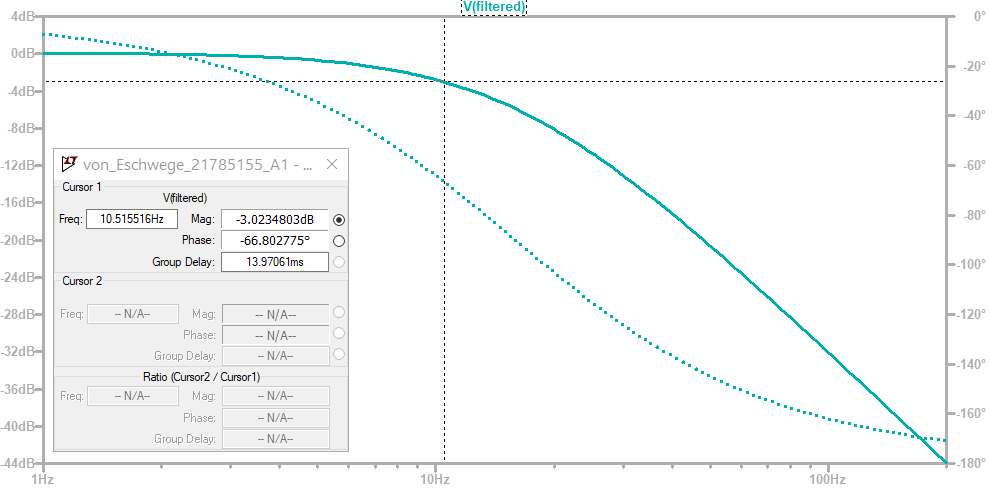
\includegraphics[width = 0.8\textwidth]{Figures/ac.png}
    \caption{Cutoff Frequency Measurement}
    \label{fig:ac}
\end{figure}